

\tikzset{every picture/.style={line width=0.75pt}} %set default line width to 0.75pt        

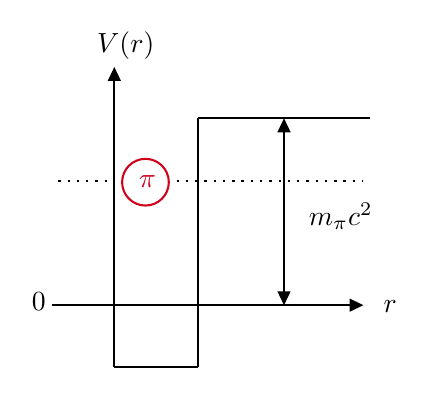
\begin{tikzpicture}[x=0.75pt,y=0.75pt,yscale=-0.75,xscale=0.75]
	%uncomment if require: \path (0,462); %set diagram left start at 0, and has height of 462
	
	%Straight Lines [id:da04487003009359902] 
	\draw    (276,240) -- (276,90) ;
	\draw [shift={(276,87)}, rotate = 90] [fill={rgb, 255:red, 0; green, 0; blue, 0 }  ][line width=0.08]  [draw opacity=0] (8.93,-4.29) -- (0,0) -- (8.93,4.29) -- cycle    ;
	%Straight Lines [id:da11984458862135328] 
	\draw    (236,240) -- (433,240) ;
	\draw [shift={(436,240)}, rotate = 180] [fill={rgb, 255:red, 0; green, 0; blue, 0 }  ][line width=0.08]  [draw opacity=0] (8.93,-4.29) -- (0,0) -- (8.93,4.29) -- cycle    ;
	%Straight Lines [id:da39644848633047847] 
	\draw    (330,280) -- (330,120) ;
	%Straight Lines [id:da23479083436400994] 
	\draw    (330,280) -- (297,280) -- (276,280) ;
	%Straight Lines [id:da22091112894519627] 
	\draw    (276,240) -- (276,280) ;
	%Straight Lines [id:da47586844464292766] 
	\draw  [dash pattern={on 0.84pt off 2.51pt}]  (240,160) -- (276,160) ;
	%Straight Lines [id:da07090607985351194] 
	\draw  [dash pattern={on 0.84pt off 2.51pt}]  (316,160) -- (436,160) ;
	%Flowchart: Connector [id:dp0772408562939938] 
	\draw  [color={rgb, 255:red, 208; green, 2; blue, 27 }  ,draw opacity=1 ] (281,161) .. controls (281,152.72) and (287.72,146) .. (296,146) .. controls (304.28,146) and (311,152.72) .. (311,161) .. controls (311,169.28) and (304.28,176) .. (296,176) .. controls (287.72,176) and (281,169.28) .. (281,161) -- cycle ;
	%Straight Lines [id:da8208549108465544] 
	\draw    (330,120) -- (440,120) ;
	%Straight Lines [id:da059140841724983684] 
	\draw    (385,237) -- (385,123) ;
	\draw [shift={(385,120)}, rotate = 90] [fill={rgb, 255:red, 0; green, 0; blue, 0 }  ][line width=0.08]  [draw opacity=0] (8.93,-4.29) -- (0,0) -- (8.93,4.29) -- cycle    ;
	\draw [shift={(385,240)}, rotate = 270] [fill={rgb, 255:red, 0; green, 0; blue, 0 }  ][line width=0.08]  [draw opacity=0] (8.93,-4.29) -- (0,0) -- (8.93,4.29) -- cycle    ;
	
	% Text Node
	\draw (263,62.4) node [anchor=north west][inner sep=0.75pt]    {$V(r)$};
	% Text Node
	\draw (447,235) node [anchor=north west][inner sep=0.75pt]    {$r$};
	% Text Node
	\draw (290,155) node [anchor=north west][inner sep=0.75pt]  [color={rgb, 255:red, 208; green, 2; blue, 27 }  ,opacity=1 ]  {$\pi $};
	% Text Node
	\draw (221,230) node [anchor=north west][inner sep=0.75pt]    {$0$};
	% Text Node
	\draw (399,172.4) node [anchor=north west][inner sep=0.75pt]    {$m_{\pi } c^{2}$};
	
	
\end{tikzpicture}